\section{Clustering 2.0}

Recall the photo categorization problem described in Worksheets 5 and 6. An instance of the problem is given by
\begin{itemize}
	\item $n$, the number of photos (numbered from 1 to $n$);
	\item $E$, a set of weighted edges, one for each pair of photos, where the weight is a similarity in the range between 0 and 1 (the higher the weight, the more similar the photos); and
	\item $c$, the desired the number of categories, where $1 \le c \le n$.
\end{itemize}

A solution to this problem is a \textit{categorization}, which we define as a partition of photos into $c$ (non-empty) sets, or categories. In the version of this problem we dealt with in class, our goal was to find the categorization that minimized the maximum inter-category edge weight. Suppose now that we change the goal of the photo categorization to \textbf{maximize the minimum intra-category edge similarity}. We call this the \textit{Max-Min Clustering Problem} (MMCP).

\begin{questions}
	\question[2] In class, we saw that an optimal greedy algorithm for minimizing the maximum inter-category edge weight was to initialize all photos in their own category and merge the photos adjacent to the highest-weight intercategory edge until we achieved the desired number of categories. Below is a greedy algorithm for MMCP, which starts with all photos in a single category and then separates two photos that are joined by a lowest-weight intracategory edge. This is repeated until we achieve the desired number of categories.

	\begin{algorithmic}
		\Function{MMCP-Greedy}{$n,E,c$}
		\Statex $\triangleright$ $n \ge 1$ is the number of photos
		\Statex $\triangleright$ $E$ is a set of edges of the form $(p,p',s)$, where $s$ is the similarity of $p$ and $p'$
		\Statex $\triangleright$ $c$ is the number of categories, $1 \le c \le n$

		\State create a list of the edges of $E$, in increasing order by similarity
		\State let $\mathcal{C}$ be the categorization with all photos in one category
		\State Num-$\mathcal{C}\gets 1$ \hspace{.5in} $\triangleright$ Initial number of categories
		\While{Num-$\mathcal{C}$ $< c$}
		\State remove the lowest-similarity edge $(p,p',s)$ from the list
		\If{$p$ and $p'$ are in the same category $S$ of $\mathcal{C}$}
		\State $\triangleright$ split $S$ into two new categories $T$ and $T'$ as follows:
		\State put $p$ in $T$
		\State put $p'$ in $T'$
		\For {each remaining $p''$ in $S$}
		\State put $p''$ in $T$ if $p''$ is more similar to $p$ than $p'$
		\State put $p''$ in $T'$ otherwise
		\EndFor
		\State $\triangleright$ now $S$ is replaced by $T$ and $T'$ in $\mathcal{C}$
		\State Num-$\mathcal{C}$ $\gets$ Num-$\mathcal{C}+1$
		\EndIf
		\EndWhile
		\State {\bf return} $\mathcal{C}$
		\EndFunction
	\end{algorithmic}

	Give and explain a 4-node counterexample to show that this greedy algorithm is not optimal (i.e., does not always produce a solution that maximizes the minimum intra-category edge weight).

	\ifsolutions\input{q1a-sol.tex}\fi

	\begin{soln}

		Let \(C = {C_1, C_2, \dots, C_c}\) be a partition of a nodes of a set \(V\) into \(c\) categories.

		An edge, \((u, v) \in E\), is \(intra-category\) if \(\exists C_i \in C\) s.t. \(u, v \in C_i\).

		An edge, \((u, v) \in E\), is \(inter-category\) if \(\exists C_i, C_j \in C, i \neq j\) s.t. \(u\in C_i\) and \(v \in C_j\).


		Consider the node structure, and we want to split this into two categories.

		\tikzset{
			node/.style={circle, draw=black, fill=blue!15, minimum size=1.2cm, font=\large},
			edge/.style={thick},
			weight/.style={fill=white, font=\small, inner sep=1pt}
		}
		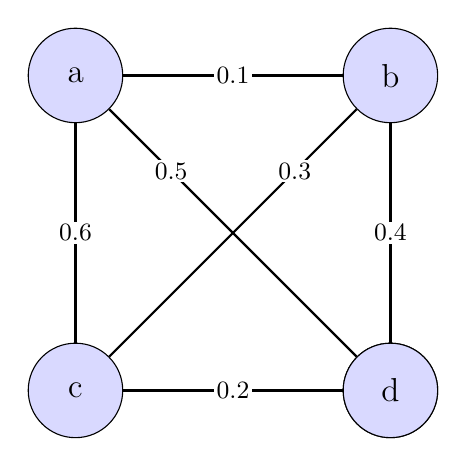
\begin{tikzpicture}

			% Define nodes in square layout
			\node[node] (a) at (0, 4) {a};
			\node[node] (b) at (4, 4) {b};
			\node[node] (c) at (0, 0) {c};
			\node[node] (d) at (4, 0) {d};
			\node[node] (e) at (4, 0) {d};

			% Draw undirected edges with weights
			\draw[edge] (a) -- (b) node[midway, weight] {0.1};
			\draw[edge] (a) -- (c) node[midway, weight] {0.6};
			\draw[edge] (a) -- (d) node[near start, weight] {0.5};
			\draw[edge] (b) -- (c) node[near start, weight] {0.3};
			\draw[edge] (b) -- (d) node[midway, weight] {0.4};
			\draw[edge] (c) -- (d) node[midway, weight] {0.2};

		\end{tikzpicture}

		Following the algorithm we get the following.

		\begin{align*}
			 & S  = \{a, b, c, d\}          & \text{ one total category initially }                                               \\
			 & T  = \{a\}, T' = \{b\}       & \text{ since } (a, b) \text{ have lowest edge weight}                               \\
			 & T  = \{a, c, d\}, T' = \{b\} & \text{ since } (c, a), (d, a) \text{ have heigher edge weight than } (c, b), (d, b) \\
			 & C = \{T, T'\}                & \text{ final collection of categories }
		\end{align*}

		Observe the min-weight intra-category edge of this collection comes from \((c, d) \in T\) with weight \(0.2\).

		But the better solution is \(T = \{a, c\}, T' = \{b, d\}\) since the min-weight edge for each, respectively is \(0.6\) and \(0.4\).

		We see that \(0.4 > 0.2\), thus the greedy algorithm fails on this four node instance when consdiering two category partion.
	\end{soln}

	\question[2] We've stated MMCP as an optimization problem. Give the decision version of MMCP, and prove that MMCP is in NP.

	\begin{soln}
		\textbf{Defintition}: We say a problem is in \(NP\) if there exists a verifier that can check in polynomial time.

		\textbf{Decision Version:}
		Does there exist a partition of \(V\) into \(c\) categories such that all intra-category edges have similarity at least \(k\), where \(0 \leq k \leq 1\)?

		\textbf{Proof that MMCP is in \(NP\):}
		To show a problem is in \(NP\), by definition, we must show that a proposed solution can be verified in polynomial time.

		A valid certificate is a partition of \(V\) into \(c\) categories \(C = \{C_1, C_2, \dots, C_c\}\). Note that \(|C| \leq n\).

		The verifier checks whether the similarity of all intra-category edges is at least \(k\).

		Let \(|V| = n\). Since the graph is complete, \(|E| = \frac{n(n-1)}{2} \in O(n^2)\).

		We provide the following Verification Algorithm:

		\begin{algorithmic}[1]
			\Procedure{Verify}{$E$, $C$, $k$}
			\For{$(u, v, s) \in E$}
			\For{$i = 1$ to $c$}
			\If{$u \in C_i$ and $v \in C_i$}
			\If{$s < k$}
			\State \Return \textbf{No}
			\EndIf
			\EndIf
			\EndFor
			\EndFor
			\State \Return \textbf{Yes}
			\EndProcedure
		\end{algorithmic}

		\textbf{Analyzing Running Time:}
		\begin{itemize}
			\item Outer loop over all edges: \(O(n^2)\)
			\item For each edge, checking all \(c \leq n\) categories for membership of \(u, v\): \(O(n)\)
		\end{itemize}
		Total running time: \(O(n^2 \cdot n) = O(n^3)\)

		Thus, the verifier runs in polynomial time, so MMCP is in \(NP\).




	\end{soln}

	\ifsolutions\input{q1b-sol.tex}\fi

	\question[4] We will now show that MMCP is NP-hard (which, together with the proof from 3.2 that MMCP is in NP, means that it is NP-complete). We do this by reducing a known NP-hard problem to it. For this problem, you must do a reduction from the graph colouring problem, which (as a decision problem) is: given a graph $G$ and a bound $k$, can we colour the vertices of $G$ using no more than $k$ colours such that no two adjacent vertices share a colour? You may assume that $k \le n$, where $n$ is the number of vertices in $G$.

	For this part of the question, you do not need to prove the correctness of your reduction (that comes next), but you should explain the reasoning behind your reduction and why it runs in polynomial time.

	\ifsolutions\input{q1c-sol.tex}\fi

	\begin{soln}

		Let an instance of graph colouring be given with graph \(G = (V, E)\) and bound \(k\). With \(|V| = n\).

		We constuct the following partition and edge set for an instance of \(MMCP\).

		For each pair \(u, v \in V\), if \((u, v) \in E\) add \((u, v, 0)\) to \(E'\), otherwise if \((u, v) \notin E\) add \((u, v, 1)\) to \(E'\).

		Then we have \(n\) photos for each \(v \in V\) with the weighted edge set \(E'\).

		We want \(c = k\) categories, and weight at least \(1\) amongst the intra-category edges. This completes the reduction.

		The goal is to force pairs of vertices that have an edge into different categories that becomes my coloring.

		So, if I give them weight \(0\) then MMCP should not want to put them into the same category since that would not be at least \(1\).

		Then this runs in polynomial time since the only thing to do is to make a copy of \(V\) and construct a new edge set \(E'\).

		The copy of \(V\) is just \(O(n)\) time, while making \(E'\) is \(O(n^2)\) since we want a complete edge set for each pair of vertices.

		Hence, overall its polynomial.

	\end{soln}

	\question[3] To prove your reduction correct, you must prove that the answer to the MMCP instance is YES if and only if the answer the answer to the graph colouring instance is YES. For this part of the question, prove that if the answer to the graph colouring instance is YES, then the answer to your reduced MMCP instance is YES.

	\ifsolutions\input{q1d-sol.tex}\fi

	\begin{soln}
		Claim: Given the reduction, Graph Colouring instance is YES \(\iff\) MMCP instance is YES.

		Proof \(\implies\): Suppose Graph Colouring instance is YES.

		Observe having weight at least \(1\) is the same as being \(1\), since similarity is between \(0\) and \(1\).

		Then \(G\) can be coloured with no more than \(k\) colours, such that no adjacent vertices share a colour.

		WLOG assume \(G\) uses \(k\) colours, if it it used less, we could partition some colour into more colours.

		Let \(f:V \to \{1, 2, \dots, k\}\) be the colouring function such that if \((u, v) \in E\) then \(f(u) \neq f(v)\).

		We show there exists partition of \(V\) to \(k\) categories so that the intra-category edges have weight \(1\).

		For each \(j = 1, 2, \dots k\) construct categories, \(C_j = \{v \in V : f(v) = j\}\).

		Now consider an arbitrary category \(C_i\) and let \(u, v \in C_i\).

		Then we have that \(f(u) = f(v) = i\). By contrapostion, this means that \((u, v) \notin E\).

		By construction, we have \((u, v, 1) \in E'\). Since \(i\) was arbitrary, then every intra-category edge is weighted at least \(1\).

		This completes the proof of this direction.





	\end{soln}

	\question[3] Now for the other direction of the if-and-only-if: prove that if the answer to the reduced MMCP instance is YES, then the answer to the original graph colouring instance is also YES.

	\ifsolutions\input{q1e-sol.tex}\fi

	\begin{soln}
		Proof \(\impliedby\):

		Assume that MMCP instance is YES.

		Then we have \(n\) photoes partitioned into \(k\) categories with all intra-category edges weight at least \(1\).

		We denote the categories by \(C_1, C_2, \dots, C_k\).

		Then define the function \(f:V \to \{1, 2, \dots, k\}\) by
		\[
			f(v) = \begin{cases}
				1 & \text{if } v \in C_1 \\
				2 & \text{if } v \in C_2 \\
				\vdots                   \\
				k & \text{if } v \in C_k
			\end{cases}
		\]

		It suffices to show that if \(f(v) = f(u)\) then \((u, v) \notin E\).

		Suppose that \(f(v) = f(u) = i\). Then \(u, v \in C_i\) for some \(i\) with \(1 \leq i \leq k\).

		Since, MMCP is YES, this means \((u, v, 1) \in E'\) as all intra-category edges are weighted at least \(1\).

		But we only added \((u, v, 1)\) to \(E'\) iff \((u, v) \notin E\). Thus, \((u, v) \notin E\) and the graph \(G\) is \(k\) colourable.

		This completes the proof.

	\end{soln}

\end{questions}
